\chapter{Existing solutions}
In this chapter we will discuss currently available solutions in our problem domain.
First, each application is briefly introduced.
Second, we state use cases by which we later compare the applications.
Last, we describe how each application fulfills these use cases.

\section{Overview of existing similar applications}
Now we will briefly introduce currently available applications.

\todo[inline]{napisat ci su jednotlive aplikacie na webe alebo stiahnutelna appka}

\subsection*{Allergy Menu}
  There are allergen icons in the menu item's description.
  A guest can interact with the menu by choosing what allergens they want to avoid.
  A guest can also select an option that they are either a vegan or vegetarian.
  The application filters out items of a menu to meet the guest's preferences.
  The application allows a restaurant employee create a menu and specify what allergens are contained in each item of the menu.

  Android and iOS app

  Information on the dishes, both public and internal information can be managed along with additional documentation, such as photographs of labelling, can ensure all allergy information is logged in one place.

  Our menu is designed to feel like your business, so you just upload your logo within the my account area.

  You can create custom categories for your menu to help users find dishes easily.

  Dished can be easily duplicated and hidden on the live system when they are not active. Allowing you to keep your menu up to date easily.

  Along with the usual allergen list, there are flags to allow the system to work for vegans and vegetarians.

  You can also add internal notes, recipes and method about each dish, with the ability to upload photographs of products used within a dish with notes for each photo, allowing you to manage your information easily.

  When creating your recipes, it also searches product information with allergen suggestions and ingredients lists to make inputting your information easier and accurate.

  Print ingredient labels onto any label printer ( 54 mm x 101 mm label) or Avery labels (14 per sheet paper), quick and easily to ensure you meet Natasha's Law.

  You can also download printed literature in the My Account area to create point of sale graphics for your menu with your unique reference and QR code, along with code to add a link from your website direct to the allergy menu.

  The system will email you every month to review your menu with all the allergy information, you can then set if the menu is up to date, or edit from there if items have changed.

  CSV import - Link up your CSV export with our system and then easily import your file as and when you need to.

  API integration - Talk to your supplier about integrating with our API, allowing them to sync your information directly into Allergy Menu without manual intervention.

  The six character restaurant code used by Allergy Menu to identify a restaurant. This is what the end user enters into the app.

  API documentation

  \begin{figure}[h]
    \centering
    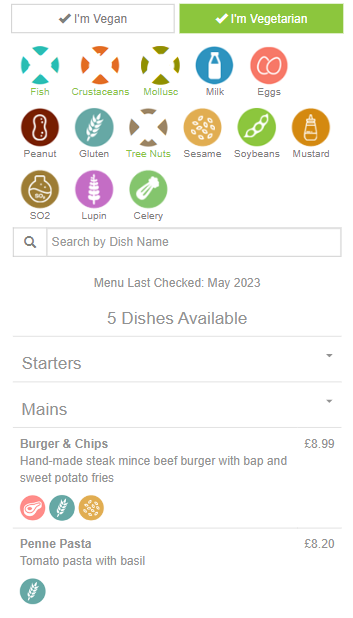
\includegraphics[width=0.62\linewidth]{master-thesis/img/existing-applications-screenshots/allergy_menu_screenshot}
    \caption{The Allergy Menu application}
  \end{figure}
% end of \subsection

\subsection*{Allergen Checker}
  Allergen Management Software

  “Educate by Allergen Checker” is a yearly subscribed licence which enables colleges in the UK to use our platform to help educate the future generation of chefs and managers.

  Simply type in all the ingredients that you use in your food products and dishes and they will be stored in your own virtual food cupboard. Add accurate information from labels or data sheets. We have included a generic list of ingredients to get you started.  

  Once you have added all your ingredients, create your dishes and save them in different categories

  Or create a QR code for ease of use to your customers.

  Our simple and clear food allergen and ingredient icons will help keep your customers informed, quickly and effectively.

  dashboard as a central point from which you can manage ingredients, categories and menus

  add banner image and logo of restaurant

  an ingredient can be raw, home made or manufactured

  you can edit ingredients

  clone ingredients

  menu is created in steps

  number of dishes per page when printing

  trace allergens: may contain

  \begin{figure}[h]
    \centering
    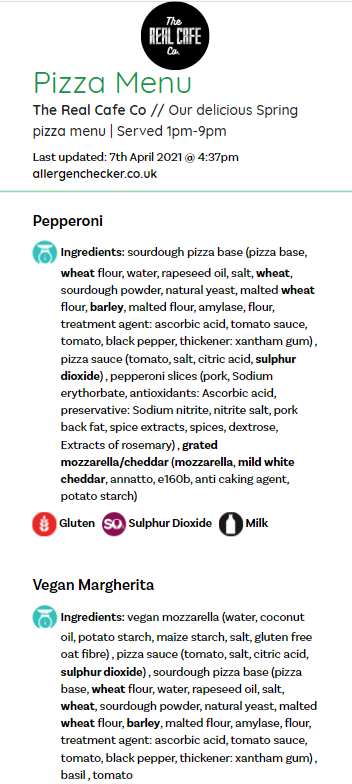
\includegraphics[width=0.62\linewidth]{master-thesis/img/existing-applications-screenshots/allergen_checker_menu_screenshot}
    \caption{The Allergen Checker application}
  \end{figure}
% end of \subsection

\subsection*{BigZpoon}
  Cloud based solution

  B2B SaaS venture

  ordering system

  Menu website can be integrated into the restaurants website

  Menu has 3 parts - ok to eat, ok to eat with modifications, not ok to eat

  The menu contains information why a menu is not ok to eat

  Detailed nutrition facts about meals

  As guest changes ingredients of what they want to eat the nutrition facts table changes too

  Guest can set nutritional goals

  App tracks nutrition of whole meal

  Can order online

  Creating a menu item comprises of specifying all modifications

  Usage analytics and insights 

  reviews (stars) of restaurants

  “Once the guests have entered their preferences, our AI driven software guides them to choose the right meal options by clearly marking the items and choices that fit their restrictions.  Further, our real-time nutrition calculator keeps accurate track of all nutritional details for chosen meal items and alerts the guest when the goals are exceeded.”

  \begin{figure}[h]
    \centering
    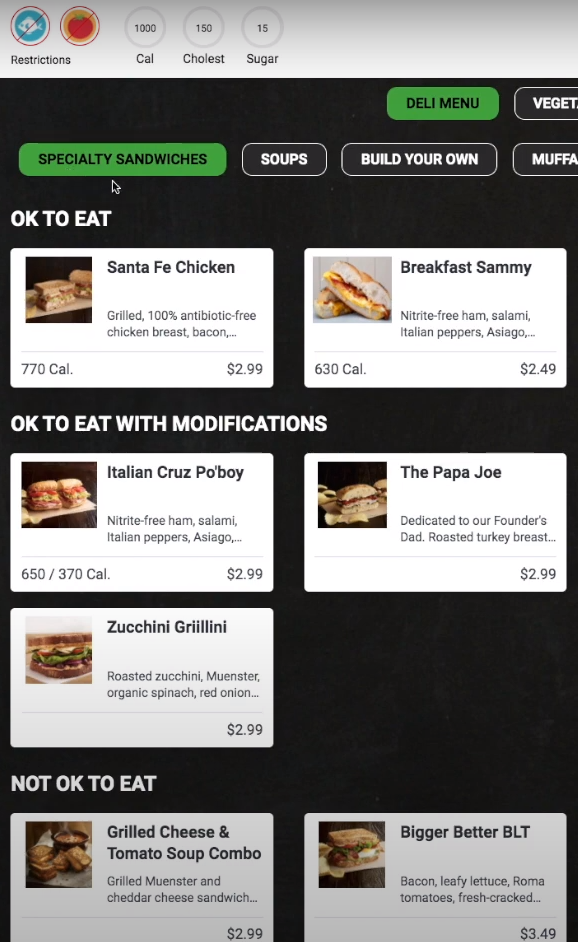
\includegraphics[width=0.62\linewidth]{master-thesis/img/existing-applications-screenshots/bigzpoon_screenshot}
    \caption{The BigZpoon application}
  \end{figure}
% end of \subsection

\subsection*{Tenkites}
  can link to existing EAS and POS system
  information to tenkites and out to every point of sale
  can be connected to social media
  optimized for search engines
  dashboard insights

  \begin{figure}[h]
    \centering
    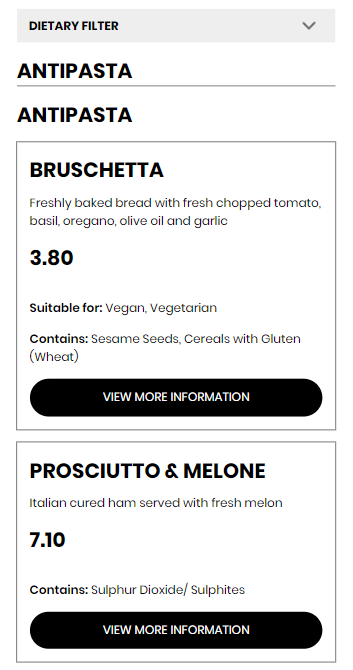
\includegraphics[width=0.62\linewidth]{master-thesis/img/existing-applications-screenshots/tenkites_menu_screenshot}
    \caption{The Tenkites application}
  \end{figure}
% end of \subsection

\subsection*{Menu Guide}
  no download of app needed

  you may choose to highlight food items that are dairy-free, vegetarian and vegan

  Additional menu choices (like halal, low-calorie, low GL) can be shown in the editable notes field.

  No internet of WiFi in your venue? No problem, simply download our offline menus app to a shared tablet (available for Android devices on Google Play) and your customers can browse your allergen menus no matter where they are!

  select allergens and the app highlights affected dishes

  \begin{figure}[h]
    \centering
    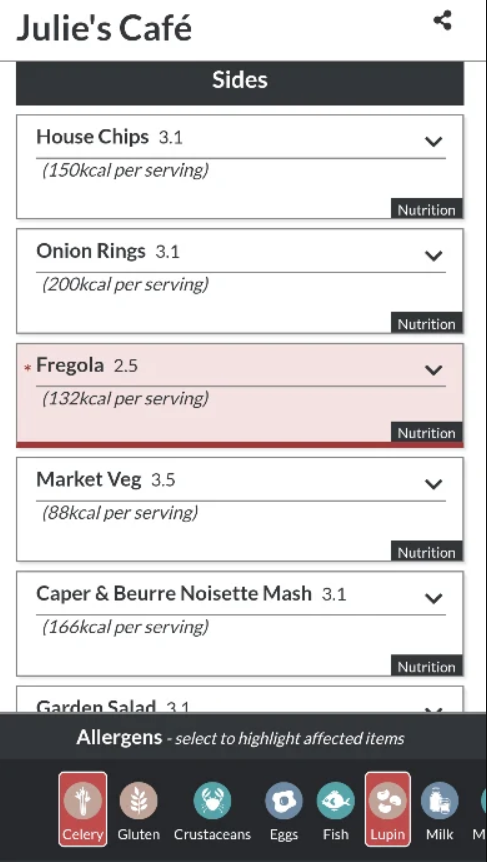
\includegraphics[width=0.62\linewidth]{master-thesis/img/existing-applications-screenshots/menu_guide_screenshot}
    \caption{The Menu Guide application}
  \end{figure}
% end of \subsection

\todo[inline]{add Hubl app and restaurantallergens.com}
% \subsection*{Hubl}  

  % \begin{figure}[h]
  %   \centering
  %   \includegraphics[width=0.62\linewidth]{master-thesis/img/existing-applications-screenshots/.png}
  %   \caption{The  application}
  % \end{figure}
% end of \subsection